\documentclass[crop,tikz]{standalone}
\usepackage{amsmath}
\usepackage{amsfonts}
\usepackage{physics}
\usepackage{tikz}
\usetikzlibrary{shapes}
\usepackage{dsfont}
\usepackage{bbm}
% parameters for the MPS drawings
\definecolor{Tcolor}{RGB}{255, 235, 171}
\definecolor{Wcolor}{RGB}{190, 190, 255}
\def\textoffsetVertical{0.8}
\def\nodewidth{0.6*28.5}
\def\legwidth{0.8}
\def\nodedistance{1.25}
\def\textoffsetVerticalW{0.9}
\def\textoffsetHorizontalW{-0.9}
\def\textoffsetVerticalMPO{1.2}
\def\yoffset{1}
\def\xoffset{3}
\def\resultMPSYoffset{2.5}
\def\resultMPSXOffsetSmall{2}
\def\resultMPSXOffset{3}
\def\dotsOffset{3}
\def\conjOffsetVertical{1.25}
\def\conjOffsetVerticalLarge{2.2}
\def\curvedLineXOffset{0.7}
\def\cmscale{28.5}
\def\miniatureScale{0.5}
\def\Heffheight{1.2*28.5}
\def\Heffwidth{4.0*28.5}
\def\Heffonewidth{3.0*28.5}
\def\miniatureTextOffsetVertical{0.5}
\begin{document}
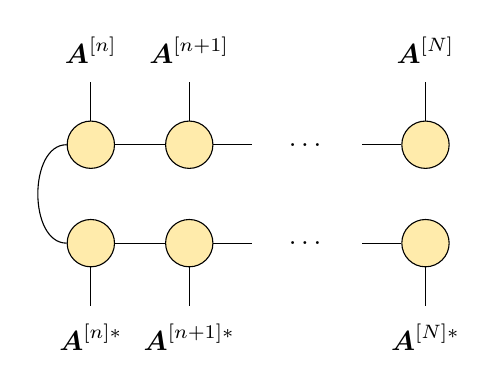
\begin{tikzpicture}[baseline=(current  bounding  box.center)]
    \node[draw, shape=circle, fill=Tcolor, minimum width=\nodewidth] (T4) at ({3*\nodedistance+1*\dotsOffset}, 0) {};
    \node[draw, shape=circle, fill=Tcolor, minimum width=\nodewidth] (T5) at ({4*\nodedistance+1*\dotsOffset}, 0) {};
    \node[draw, shape=circle, fill=Tcolor, minimum width=\nodewidth] (T6) at ({4*\nodedistance+2*\dotsOffset}, 0) {};

    \node[draw, shape=circle, fill=Tcolor, minimum width=\nodewidth] (T4c) at ({3*\nodedistance+1*\dotsOffset}, -\conjOffsetVertical) {};
    \node[draw, shape=circle, fill=Tcolor, minimum width=\nodewidth] (T5c) at ({4*\nodedistance+1*\dotsOffset}, -\conjOffsetVertical) {};
    \node[draw, shape=circle, fill=Tcolor, minimum width=\nodewidth] (T6c) at ({4*\nodedistance+2*\dotsOffset}, -\conjOffsetVertical) {};

    \draw (T4) -- (T5);
    \draw (T4) -- ++(0, \legwidth);
    \draw (T5) -- ++(0, \legwidth);
    \draw (T5) -- ++(\legwidth, 0);
    \draw (T6) -- ++(0, \legwidth);
    \draw (T6) -- ++(-\legwidth, 0);

    \draw (T4c) -- (T5c);
    \draw (T4c) -- ++(0, -\legwidth);
    \draw (T5c) -- ++(0, -\legwidth);
    \draw (T5c) -- ++(\legwidth, 0);
    \draw (T6c) -- ++(0, -\legwidth);
    \draw (T6c) -- ++(-\legwidth, 0);

    \draw (T4) to[in=180, out=180, looseness = 1] (T4c);

    \node[] (dots1) at ({4*\nodedistance+1.5*\dotsOffset}, 0) {$\dots$};
    \node[] (dots1) at ({4*\nodedistance+1.5*\dotsOffset}, -\conjOffsetVertical) {$\dots$};

    \node[] (text4) at ({3*\nodedistance+1*\dotsOffset}, \textoffsetVertical+\legwidth/2) {$\vb*{A}^{[n]}$};
    \node[] (text5) at ({4*\nodedistance+1*\dotsOffset}, \textoffsetVertical+\legwidth/2) {$\vb*{A}^{[n+1]}$};
    \node[] (text6) at ({4*\nodedistance+2*\dotsOffset}, \textoffsetVertical+\legwidth/2) {$\vb*{A}^{[N]}$};

    \node[] (text4) at ({3*\nodedistance+1*\dotsOffset}, -\conjOffsetVertical-\textoffsetVertical-\legwidth/2) {$\vb*{A}^{[n]*}$};
    \node[] (text5) at ({4*\nodedistance+1*\dotsOffset}, -\conjOffsetVertical-\textoffsetVertical-\legwidth/2) {$\vb*{A}^{[n+1]*}$};
    \node[] (text6) at ({4*\nodedistance+2*\dotsOffset}, -\conjOffsetVertical-\textoffsetVertical-\legwidth/2) {$\vb*{A}^{[N]*}$};
\end{tikzpicture}
\end{document}